%!TEX root = ../presentation.tex

\tikzset{
  event/.style={
    draw,
    inner sep=0pt,
    circle,
    minimum width=4mm
  },
  events/.style={
    xscale=.8,
    yscale=.6,
    shorten >=0pt
  },
  unit/.style={
    event,
    path picture={ 
      \draw[black]
        (path picture bounding box.south east) -- (path picture bounding box.north west)
        (path picture bounding box.south west) -- (path picture bounding box.north east);
    }
  },
  small unit/.style={
    unit,
    minimum width=2.5mm
  }
}

\providecommand{\signaldx}{.15}
\providecommand{\signaldy}{.35}
%\firstbar{color}{(x,y)}{length}{caption}
\providecommand{\firstbar}[4]{
  \pgfmathsetmacro{\signallength}{#3-\signaldx}
  \filldraw[draw=black,fill=#1]
    #2 ++(0,\signaldy) -- ++(\signallength,0) -- ++(\signaldx,-\signaldy)
    --++(-\signaldx,-\signaldy) -- ++(-\signallength,0) -- cycle;
  \pgfmathsetmacro{\halflength}{.5*#3}
  \path #2 ++(\halflength,0) node {#4};
}
%\midbar{color}{(x,y)}{length}{caption}
\providecommand{\midbar}[4]{
  \pgfmathsetmacro{\signallength}{#3-2*\signaldx}
  \filldraw[draw=black,fill=#1]
    #2 -- ++(\signaldx,\signaldy) --++(\signallength,0) --++(\signaldx,-\signaldy)
    --++(-\signaldx,-\signaldy) --++(-\signallength,0) -- cycle;
  \pgfmathsetmacro{\halflength}{.5*#3}
  \path #2 ++(\halflength,0) node {#4};
}
%\lastbar{color}{(x,y)}{length}{caption}
\providecommand{\lastbar}[4]{
  \pgfmathsetmacro{\signallength}{#3-\signaldx}
  \fill[#1]
    #2 -- ++(\signaldx,\signaldy) -- ++(\signallength,0) --++(0,-\signaldy)
    --++(0,-\signaldy) --++(-\signallength,0) -- cycle;
  \draw[black]
    #2 -- ++(\signaldx,\signaldy) -- ++(\signallength,0)
    #2 -- ++(\signaldx,-\signaldy) -- ++(\signallength,0);
  \pgfmathsetmacro{\halflength}{.5*#3}
  \path #2 ++(\halflength,0) node {#4};
}
%\onlybar{color}{(x,y)}{length}{caption}
\providecommand{\onlybar}[4]{
  \pgfmathsetmacro{\signallength}{#3}
  \fill[#1]
    #2 ++(0,\signaldy) -- ++(\signallength,0) -- ++(0,-\signaldy) 
    --++(0,-\signaldy) -- ++(-\signallength,0);
  \draw
    #2 -- ++(0,\signaldy) -- ++(\signallength,0) ++(0,-\signaldy) 
    ++(0,-\signaldy) -- ++(-\signallength,0) -- #2;
  \pgfmathsetmacro{\halflength}{.5*#3}
  \path #2 ++(\halflength,0) node {#4};
}

\chapter{Hardware SRV with Embedded Tracing Units}
\label{chap_rv}
\targets{
  \item See the state of the art and current research in the field of verification using embedded tracing units.
  \item See how program flow trace reconstruction and lightweight instrumentation work.
  \item See how to write TeSSLa specifications for an embedded system.
}

\section{Hardware Monitoring}

\subsection[Interactive Workflow]{Interactive Hardware Monitoring Workflow}
%!TEX root = ../../presentation.tex

\begin{frame}{State of the Art Hardware Monitoring / Debugging}
  \begin{itemize}
    \item Embedded, hybrid and cyber-physical systems have
      \alert{tight time and resource constraints}.
    \item Comprehensive \alert{logging} output in the software (e.g. via instrumentation)  \alert{decreases the performance} significantly.
    \item \alert{Breakpoint}-based debugging features of the processor \alert{are slow}
      due to the potentially high number of interruptions.
    \item Logging and breakpoints are \alert{highly intrusive}.\\
      Problematic for \alert{concurrent programs} or \alert{real-time} applications.
  \end{itemize}
\end{frame}

\begin{frame}[plain]{Embedded Tracing Unit: ARM CoreSight}
  \textwidthplain

  \begin{columns}
    \column{5cm}
    \uncover<2>{
      \vskip3ex

      \inhead{DSTREAM}

      \begin{itemize}
        \item Record trace for offline\\
          reconstruction and analysis.
        \item Traces can be recorded for\\
          at most a few seconds.
        \item Trace buffer of 4GB for\\
          a recording speed of 10 Gbit/s.
      \end{itemize}

      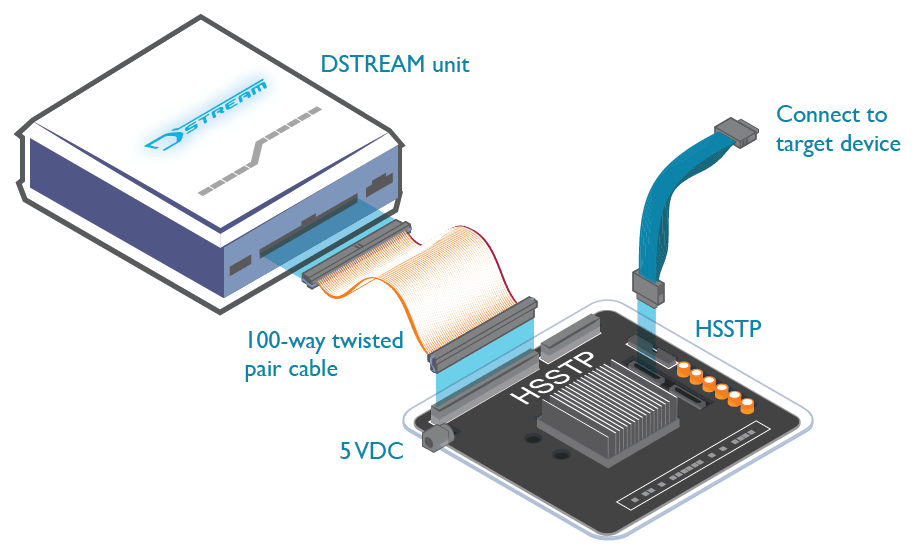
\includegraphics[width=5cm]{content/chapter_hardware_srv/dstream}
    }

    \column{6cm}
    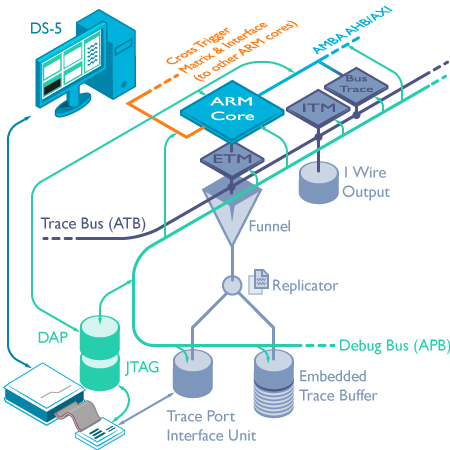
\includegraphics[width=6cm]{content/chapter_hardware_srv/coresight}
  \end{columns}
\end{frame}

\begin{frame}{Interactive Hardware Monitoring Workflow}
  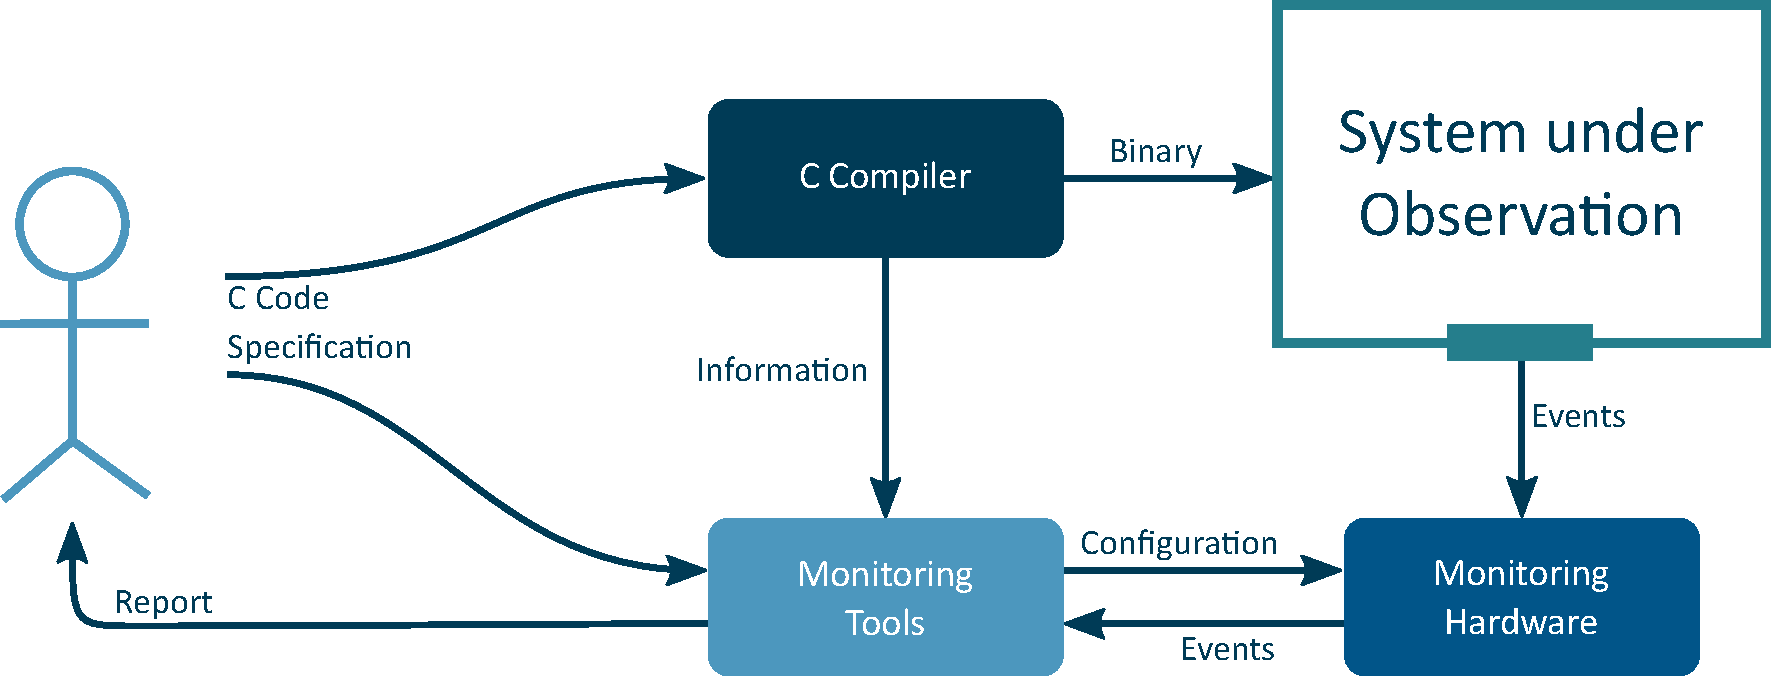
\includegraphics[width=\textwidth]{content/chapter_hardware_srv/overview-workflow.pdf}

  \vskip3ex\pause

  \alert{\large Fast reconfigurablility for interactive debugging sessions}

  \vskip3ex

  \begin{columns}
    \column{4.5cm}
    \inhead{Synthesized FPGA design}

    \begin{itemize}
      \item Trace Reconstruction\\\strut
      \item Monitoring Engine
    \end{itemize}

    \column{5cm}
    \inhead{configured through memory with}

    \begin{itemize}
      \item program binary\\
        (LUT of jumps)\strut
      \item monitoring specification
    \end{itemize}
  \end{columns}
\end{frame}

\begin{frame}
  \begin{center}
    \vskip-3ex
    
\includegraphics[width=7cm]{content/chapter_hardware_srv/logos/coems}

    \vskip1ex

    \raisebox{-0.5\height}{
\includegraphics[width=4cm]{content/chapter_hardware_srv/logos/isp-uni-luebeck}}
    \qquad
    \raisebox{-0.5\height}{
\includegraphics[width=4cm]{content/chapter_hardware_srv/logos/accemic}}

    \vskip1ex

    \raisebox{-0.5\height}{
\includegraphics[width=4cm]{content/chapter_hardware_srv/logos/airbus}}
    \qquad
    \raisebox{-0.5\height}{
\includegraphics[width=4cm]{content/chapter_hardware_srv/logos/hvl}}
    
    \vskip1ex

    
\includegraphics[width=4cm]{content/chapter_hardware_srv/logos/thales}
  \end{center}
\end{frame}

\begin{frame}{COEMS Hardware}
  \includegraphics[width=\textwidth]{content/chapter_hardware_srv/coems-hardware.pdf}
\end{frame}

\begin{frame}{COEMS Advantages}
  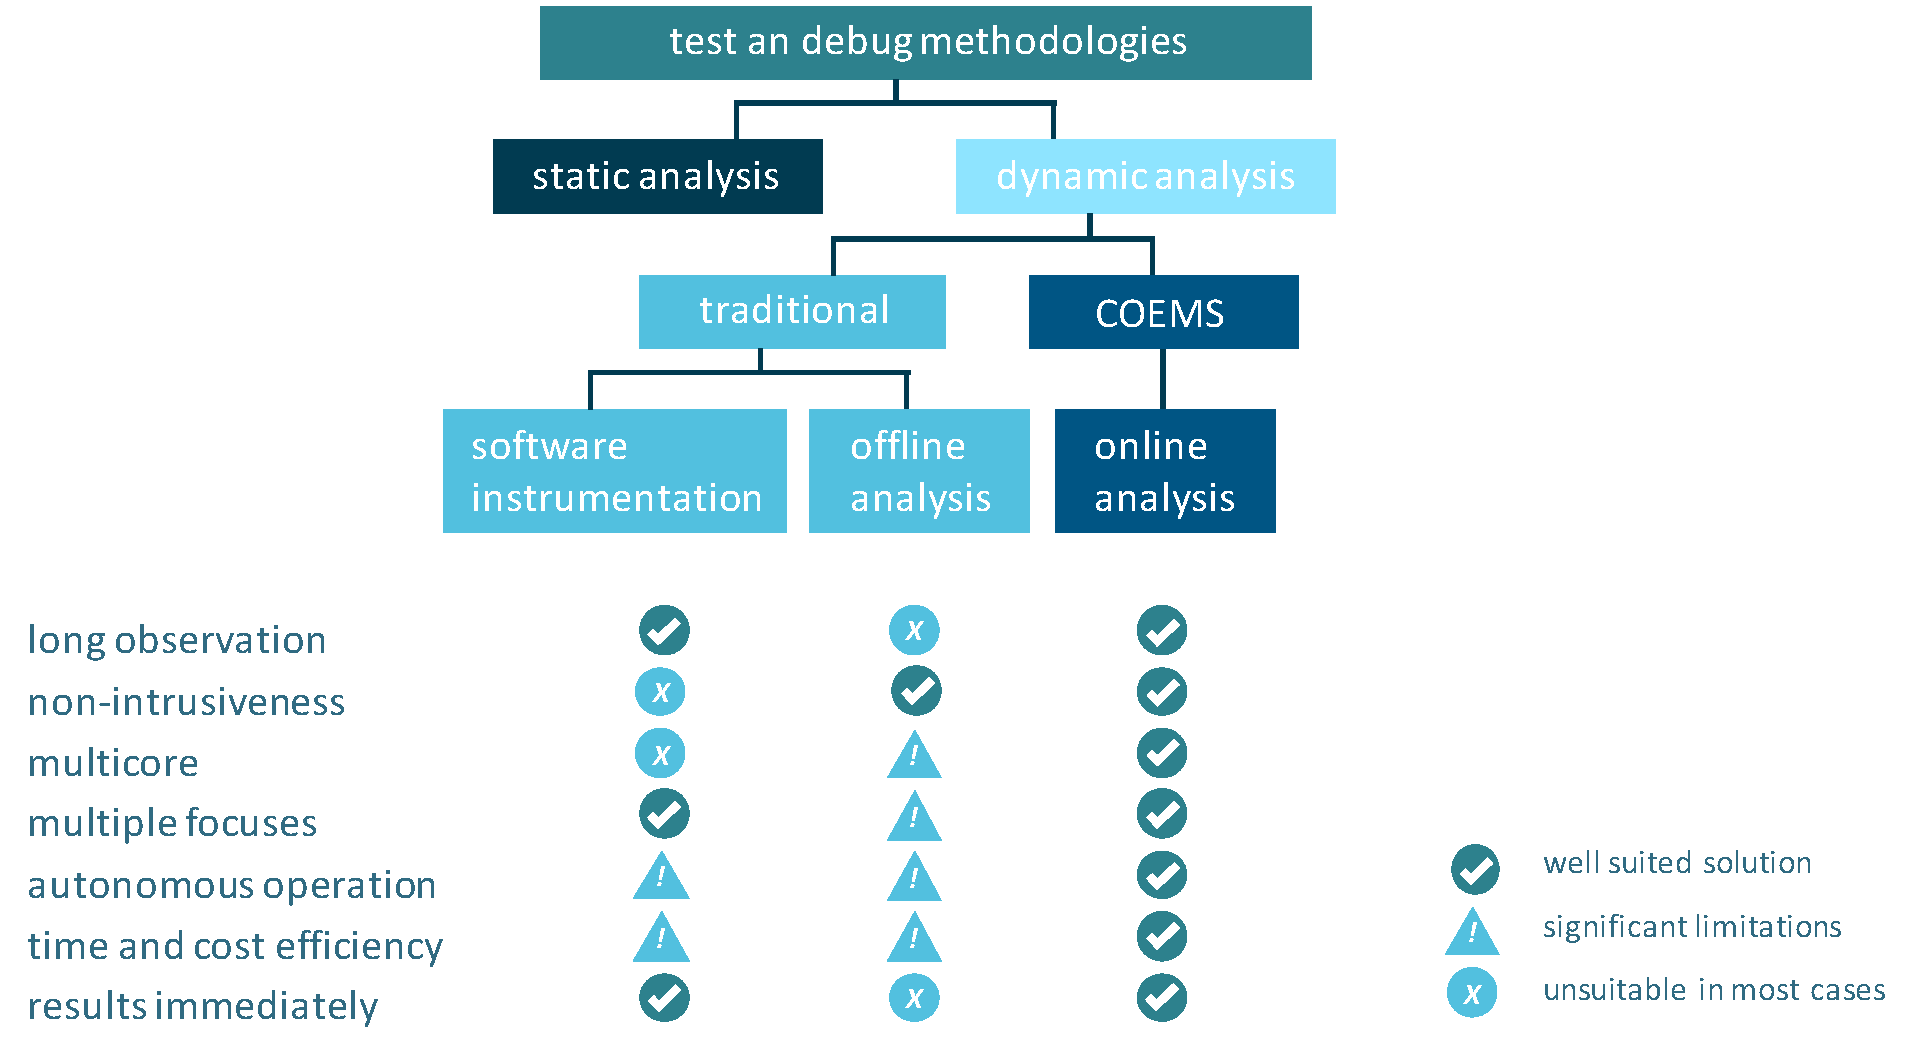
\includegraphics[width=\textwidth]{content/chapter_hardware_srv/coems-advantages.pdf}
\end{frame}

\subsection[Program Flow]{Monitoring Program Flow Trace}
%!TEX root = ../../presentation.tex

\begin{frame}[plain]{Monitoring Program Flow Trace: Tools}
  \textwidthplain
  \centering
  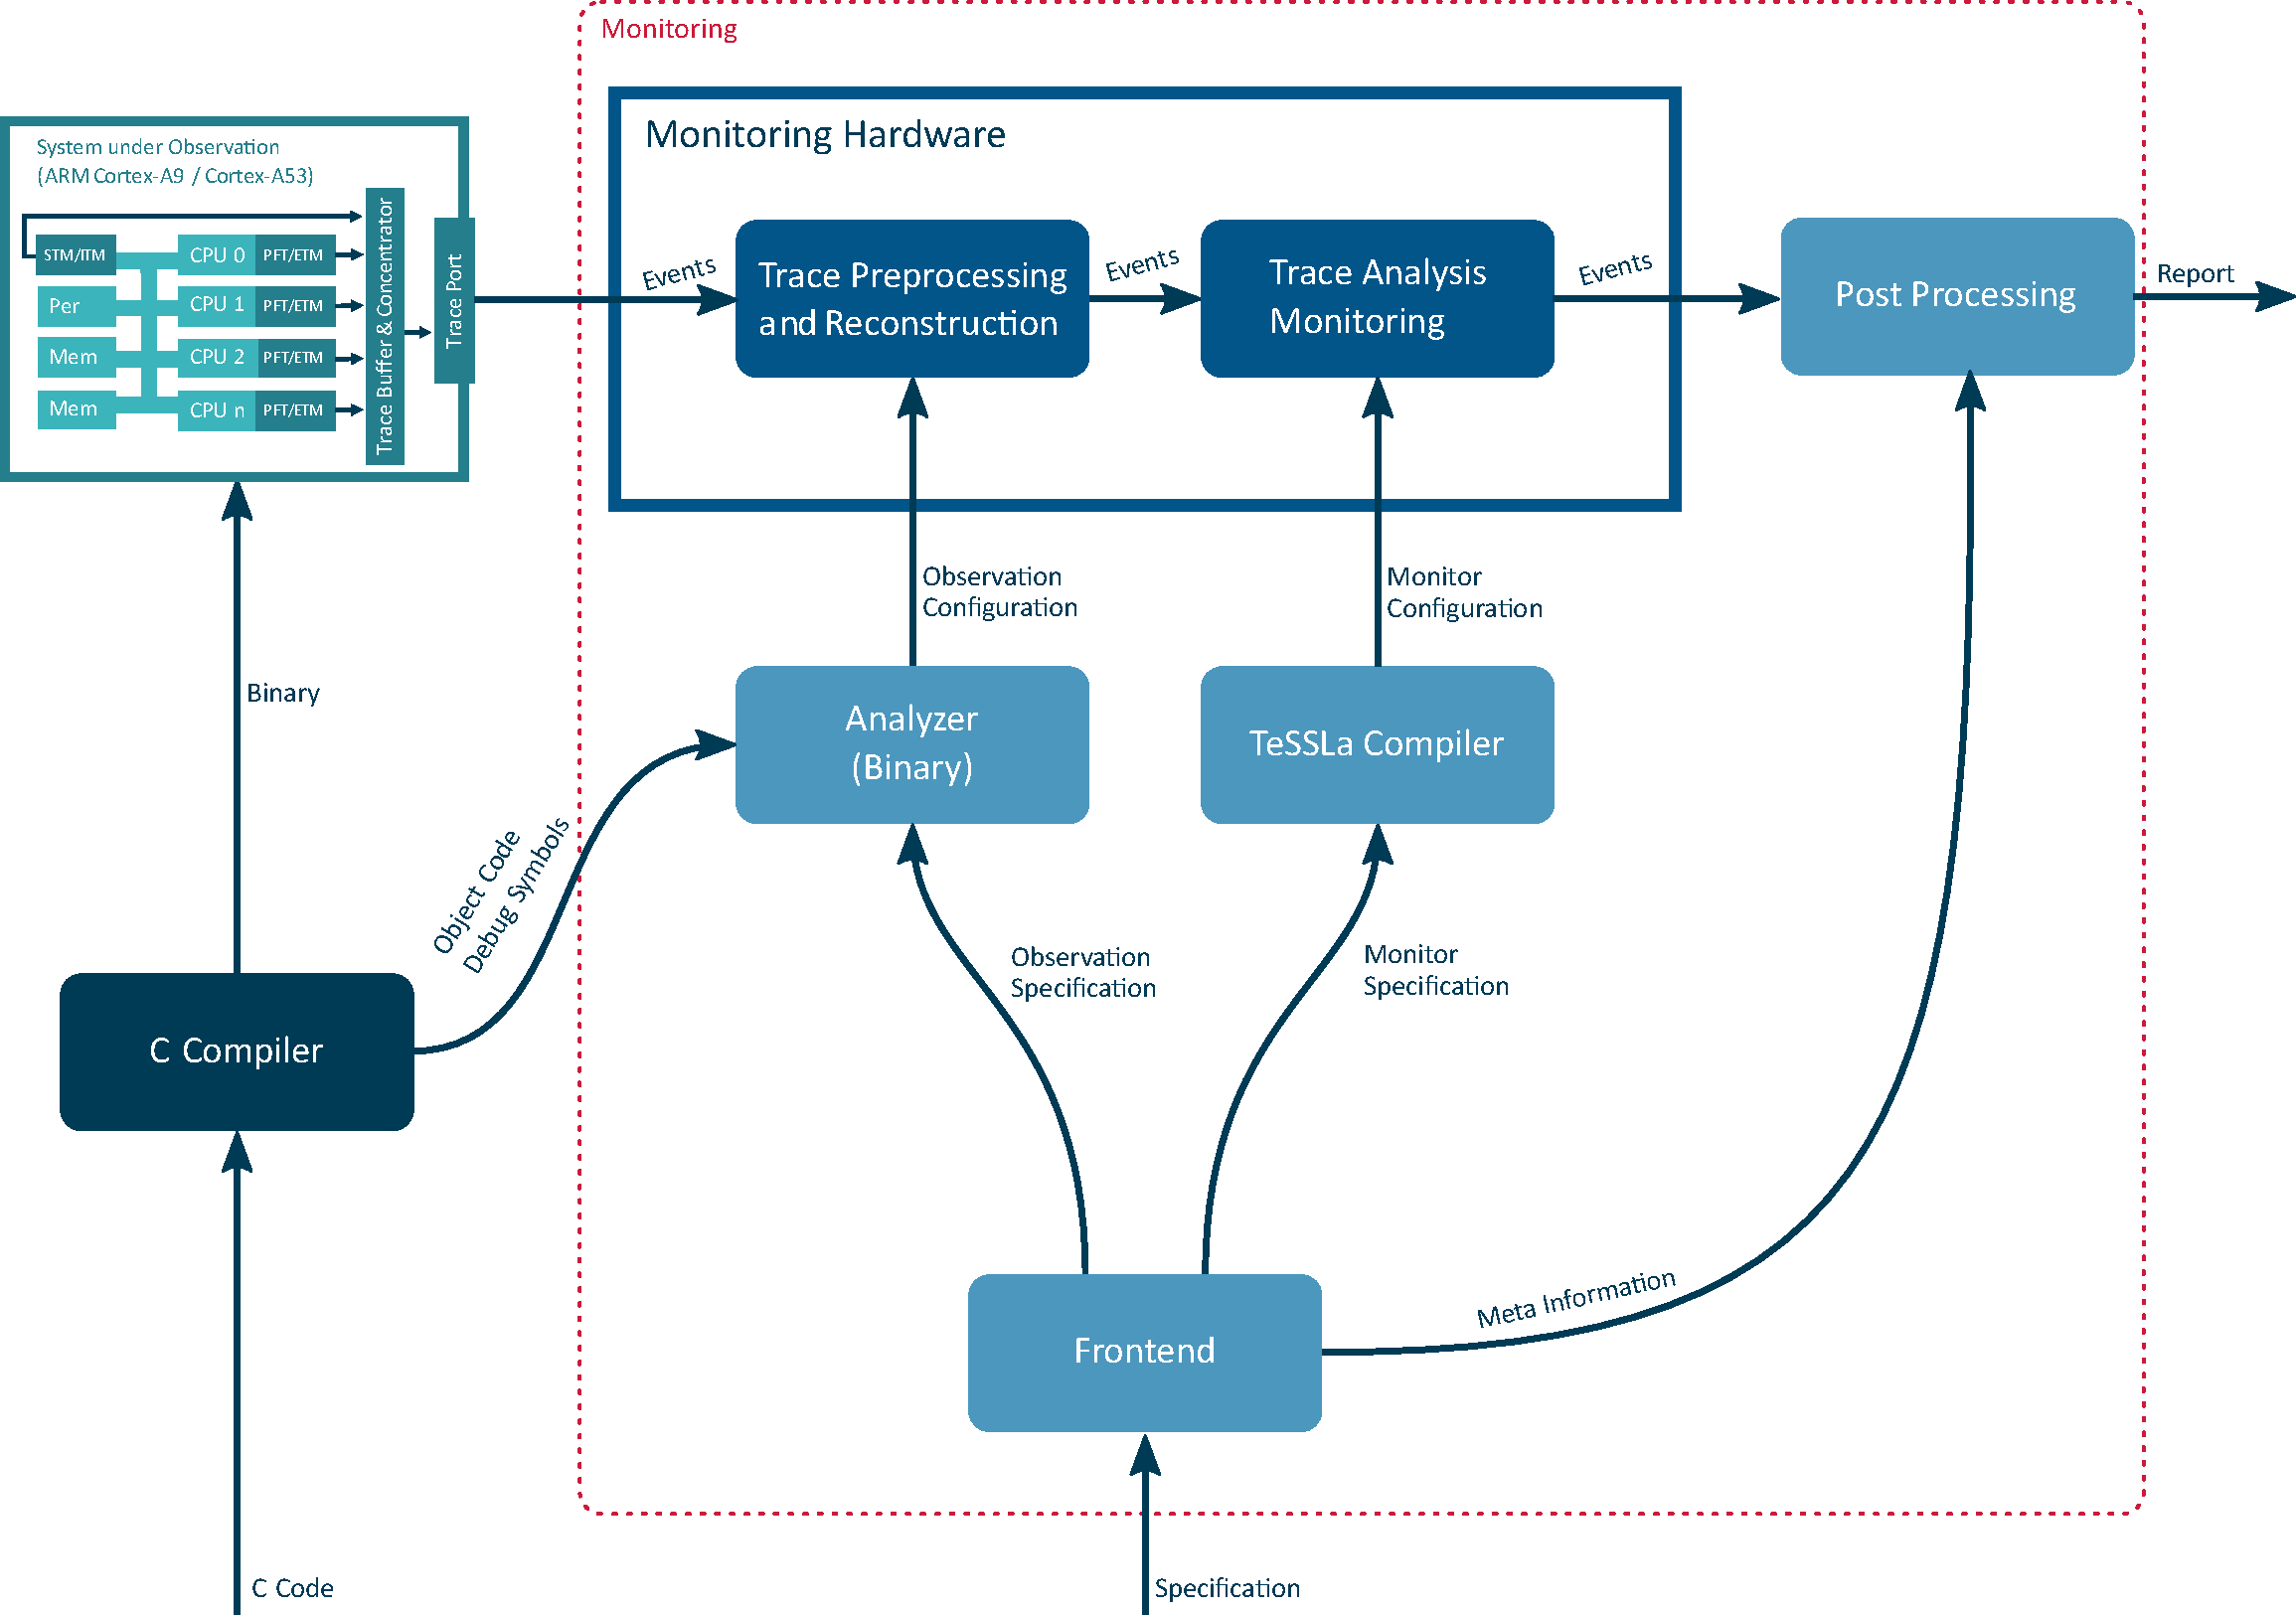
\includegraphics[width=.9\textwidth]{content/chapter_hardware_srv/overview-program-trace.pdf}
\end{frame}

\begin{frame}[t,plain,fragile]{Trace Reconstruction}
  \textwidthplain
  \vskip-4ex
  \hfill
  \tikzset{
    L1/.style={},
    L1a/.style={},
    L1b/.style={},
    L2/.style={},
    L3/.style={},
    L1no/.style={},
    L1yes/.style={},
    L1ano/.style={},
    L1ayes/.style={},
    L1byes/.style={},
    L2yes/.style={},
    active node/.style={draw=alertedcolor,fill=alertedcolor!18},
    active edge/.style={alertedcolor}
  }
  \newcommand{\highlight}[2]{\uncover<#1->{\alt<#1>{\colorbox{alertedcolor!18}{\strut #2}}{\colorbox{white}{\strut #2}}}}
  \newcommand{\highlightEmpty}[1]{\uncover<#1->{\colorbox{white}{\strut}}}
  \only<2>{\tikzstyle{L1}=[active node]}
  \only<3>{\tikzstyle{L1a}=[active node]\tikzstyle{L1no}=[active edge]}
  \only<4>{\tikzstyle{L1b}=[active node]\tikzstyle{L1ano}=[active edge]}
  \only<5>{\tikzstyle{L1}=[active node]\tikzstyle{L1byes}=[active edge]}
  \only<6>{\tikzstyle{L1a}=[active node]\tikzstyle{L1no}=[active edge]}
  \only<7>{\tikzstyle{L2}=[active node]\tikzstyle{L1ayes}=[active edge]}
  \only<8>{\tikzstyle{L1}=[active node]\tikzstyle{L2yes}=[active edge]}
  \only<9>{\tikzstyle{L3}=[active node]\tikzstyle{L1yes}=[active edge]}
  \begin{tikzpicture}[
      every node/.style={inner sep=1pt, font=\small},
      every state/.append style={inner sep=0pt, minimum size=22pt},
      shorten >=1pt,
      auto, thick, node distance=-1mm and 15mm
    ]
    \node[state, initial, L1] (L1) {L1};
    \node[state, right=8mm of L1, L1a] (L1a) {L1a};
    \node[state, above right=of L1a, L1b] (L1b) {L1b};
    \node[state, below right=of L1a, L2] (L2) {L2};
    \node[state, below=5mm of L1, L3] (L3) {L3};

    \path[->]
      (L1) edge[L1yes] node[swap] {yes} (L3)
      (L1) edge[L1no] node {no} (L1a)
      (L1a) edge[L1ayes, bend right=10] node[near end, swap] {yes/odd} (L2)
      (L1a) edge[L1ano, bend left=10] node[near end] {no/even} (L1b)
      (L1b) edge[L1byes, bend right=60, looseness=.5] node[swap, near start] {yes} (L1)
      (L2) edge[L2yes, bend left=60, looseness=.5] node[near start] {yes} (L1);
  \end{tikzpicture}

  \lstset{basicstyle=\ttfamily\scriptsize}

  \begin{columns}[t]
    \column{3.3cm}
    \inhead{C Code}
    \vskip-2pt
    \begin{lstlisting}[
        gobble=6,
        language=C,
        linebackgroundcolor={%
          \btLstHL<1>{}%
          \btLstHL<2>{2}%
          \btLstHL<3>{5}%
          \btLstHL<4>{9-10}%
          \btLstHL<5>{2}%
          \btLstHL<6>{5}%
          \btLstHL<7>{12-13}%
          \btLstHL<8>{2}%
          \btLstHL<9>{}%
        }]

      while (n > 1) {


        if (n % 2 == 0) {



          // even
          n = n / 2;
        } else {
          // odd
          n = 3 * n + 1;
        }
      }
    \end{lstlisting}

    \column{3.3cm}
    \inhead{Assembler}
    \vskip-2pt
    \begin{lstlisting}[
        gobble=6,
        language={},
        morekeywords={cmp,ble,bne,b},
        morekeywords={[2]L1,L1a,L1b,L2,L3},
        linebackgroundcolor={%
          \btLstHL<1>{}%
          \btLstHL<2>{2-3}%
          \btLstHL<3>{5-7}%
          \btLstHL<4>{9-10}%
          \btLstHL<5>{2-3}%
          \btLstHL<6>{5-7}%
          \btLstHL<7>{12-14}%
          \btLstHL<8>{2-3}%
          \btLstHL<9>{}%
        }]
      .L1:
            cmp $n, 1
            ble .L3
      .L1a:
            $tmp = $n % 2
            cmp $tmp, 0
            bne .L2
      .L1b:
            $n = $n / 2
            b .L1
      .L2:
            $n = 3 * $n
            $n = $n + 1
            b .L1
      .L3:
    \end{lstlisting}

    \column{1cm}
    \inhead{Branch\\taken?\\[1ex]}

    \highlight{3}{no}\\[-1ex]
    \highlight{4}{no}\\[-1ex]
    \highlight{5}{yes}\\[-1ex]
    \highlight{6}{no}\\[-1ex]
    \highlight{7}{yes}\\[-1ex]
    \highlight{8}{yes}\\[-1ex]
    \highlight{9}{yes}

    \column{1cm}
    \inhead{Events\\~\\[1ex]}

    \highlightEmpty{3}\\[-1ex]
    \highlight{4}{even}\\[-1ex]
    \highlightEmpty{5}\\[-1ex]
    \highlightEmpty{6}\\[-1ex]
    \highlight{7}{odd}
  \end{columns}
\end{frame}

\begin{frame}{Multithreading}
  \inhead{Problem: Distinguish multiple threads}
  \begin{itemize}
    \item We can only \alert{distinguish instructions} traced from\\ \alert{different cores}.
    \item Scheduler can execute \alert{multiple threads\\ on the same core}.
    \item Context switch reconfigures MMU\\
      \alert{$\Longrightarrow$ Same logical addresses used in different threads.}
  \end{itemize}

  \vskip3ex

  \inhead{Solution: Context ID Register}
  \begin{enumerate}
    \item OS writes \alert{thread ID} to \alert{context ID register}.
    \item Tracing unit generates \alert{context ID message}.
    \item Trace reconstruction \alert{changes lookup table}\\
      for the program flow reconstruction information.
  \end{enumerate}
\end{frame}


\section[Example Scenario]{Example Scenario: Punktförmige Zugbeeinflussung}
%!TEX root = ../../presentation.tex

\begin{frame}[plain]{\hbox{Example Scenario: Punktförmige Zugbeeinflussung}}
  \textwidthplain
  \begin{tikzpicture}
    \node (tracks) {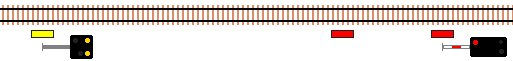
\includegraphics[width=10cm]{content/chapter_hardware_srv/pzb}};
    \path (tracks.south west)
      ++(0,-3mm) node[coordinate] (start) {}
      ++(9.5mm,0) node[coordinate] (vor) {}
        node[below=3pt] {250}
        node[above=1.8cm,text width=1cm,align=center] {distant\\signal}
      ++(5.85cm,0) node[coordinate] (magnet) {}
        node[below=3pt] {1000}
        node[above=1.8cm,text width=3cm,align=center] {500-Hz\\speed limiter}
      ++(1.93cm,0) node[coordinate] (haupt) {}
        node[below=3pt] {1250}
        node[above=1.8cm,text width=1cm,align=center] {stop\\signal}
      ++(5mm,0) node[coordinate] (ende) {}
        node[right] {pos. [m]};
    \path[thick]
      (start) edge (vor)
      (vor) edge[|-] (magnet)
      (magnet) edge[|-] (haupt)
      (haupt) edge[|->] (ende);
  \end{tikzpicture}
\end{frame}

\newcommand{\exampleSetup}{
  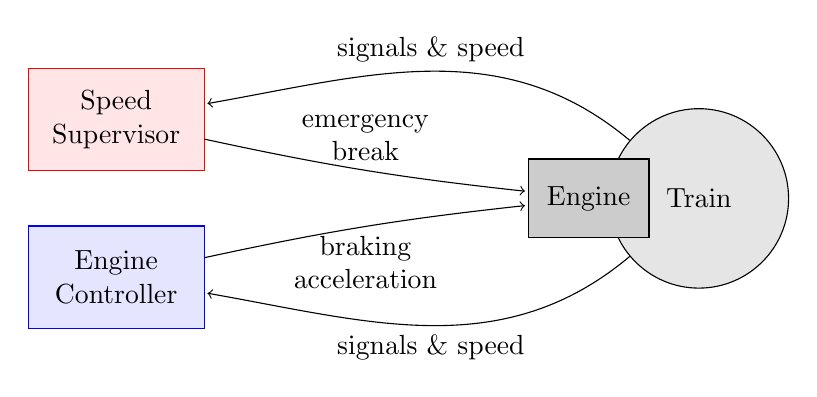
\begin{tikzpicture}[
    controller/.style={
      draw=blue,
      fill=blue!10,
      text width=2cm,
      minimum height=1.3cm,
      align=center
    },
    supervisor/.style={
      draw=red,
      fill=red!10,
      text width=2cm,
      minimum height=1.3cm,
      align=center
    },
    engine/.style={
      draw,
      fill=black!20,
      text width=1.3cm,
      minimum height=1cm,
      align=center
    },
    environment/.style={
      draw,
      circle,
      fill=black!10,
      text width=2cm,
      align=center
    }
  ]
    \node[supervisor] (supervisor) at (0,2) {Speed\\Supervisor};
    \node[controller] (controller) at (0,0) {Engine\\Controller};
    \node[environment] (environment) at (7.4,1) {Train};
    \node[engine] (engine) at (6,1) {Engine};

    \path[->, shorten >=1pt]
      (controller) edge[bend left=3] node[below] {\shortstack{braking\\acceleration}} (engine)
      (supervisor) edge[bend right=3] node[above] {\shortstack{emergency\\break}} (engine)
      (environment) edge[out=-140, in=-10] node[below] {signals \& speed} (controller)
                    edge[out=140, in=10] node[above] {signals \& speed} (supervisor);
  \end{tikzpicture}
}

\begin{frame}{Example Scenario: Braking a Train}
  \centering
  \exampleSetup
\end{frame}

\begin{frame}[t]{Example Scenario}
  \vskip-6mm\hfill
  \scalebox{.5}{\exampleSetup}
  \vskip4mm

  \centering
  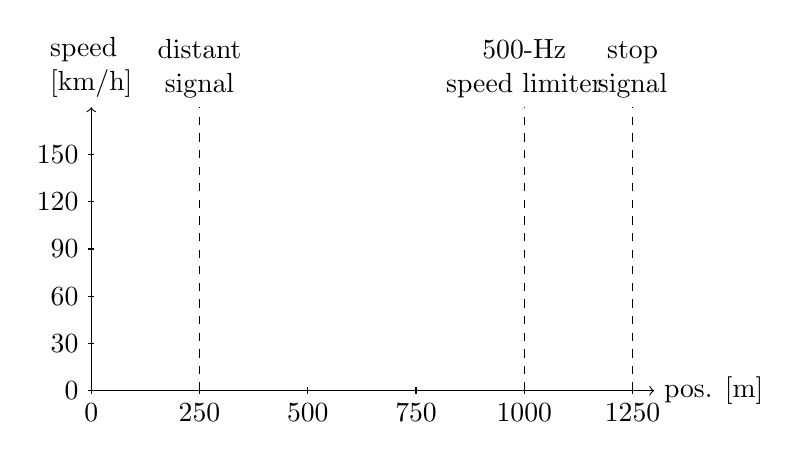
\begin{tikzpicture}[xscale=0.55,yscale=2]
    \foreach \x/\label in {2.5/distant\\signal,10/500-Hz\\speed limiter,12.5/stop\\signal} {
      \draw[dashed] (\x,0) -- (\x,1.8) node[above,text width=2cm,align=center] {\label} ;
    }
    \draw[red] plot file {content/chapter_hardware_srv/allowed_speed.table};
    \draw[blue] plot file {content/chapter_hardware_srv/speed.table};
    \draw[->] (0,0) -- (13,0) node[right] {pos. [m]};
    \draw[->] (0,0) -- (0,1.8) node[above] {\shortstack[l]{speed\\{[km/h]}}};
    \foreach \y/\label in {0/0,.3/30,.6/60,.9/90,1.2/120,1.5/150} {
      \draw (-2pt,\y) node[left] {\label} -- (2pt,\y);
    }
    \foreach \x/\label in {0/0,2.5/250,5/500,7.5/750,10/1000,12.5/1250} {
      \draw (\x,-.6pt) node[below] {\label} -- (\x,.6pt);
    }
  \end{tikzpicture}
\end{frame}

\section{Writing Specifications}

\subsection[Timing]{Measuring Timing Constraints}
%!TEX root = ../../presentation.tex

\begin{frame}[t,fragile]{Timing Constraints}{Measuring Runtime}
  \small

  \begin{block}{Property}
    Measure the runtime of one execution of the speed supervisor.
  \end{block}

  \scriptsize

  \begin{lstlisting}[gobble=4,language=tessla]
    # specify events of interest
    def call := function_call("supervisor")
    def return := function_return("supervisor")

    # specify property over the events
    def supervisorRuntime := runtime(call, return)
  \end{lstlisting}

  \pause\vskip3ex

  \inhead{TeSSLa standard library}
  \begin{lstlisting}[gobble=4,language=tessla]
    def runtime(call: Events[Unit], return: Events[Unit]) :=
      at(return, time(return) - time(call))

    def at[A,B](trigger: Events[A], values: Events[B]) :=
      filter(values, time(trigger) == time(values))
  \end{lstlisting}
\end{frame}

\begin{frame}[t,fragile]{Timing Constraints}{Aggregate Statistics}
  \small

  \begin{block}{Property}
    Measure the \emph{maximal} runtime of the speed supervisor.
  \end{block}

  \scriptsize

  \begin{lstlisting}[gobble=4,language=tessla]
    def maxSupervisorRuntime := max(supervisorRuntime)
  \end{lstlisting}

  \pause\xxx

  \inhead{TeSSLa standard library}

  \begin{lstlisting}[gobble=4,language=tessla]
    # Return the event-wise maximum of two integer streams
    def maximum(a: Events[Int], b: Events[Int]) :=
      if a > b then a else b
  
    # Aggregate the maximal event value of a given stream
    def max(x: Events[Int]) := {
      def result := merge(maximum(last(result, x), x), 0)
      result
    }
  \end{lstlisting}
\end{frame}

\begin{frame}[fragile]{Alternative Definition of Max Using Fold}
  \scriptsize
  \begin{lstlisting}[gobble=4,language=tessla]
    # Aggregate all events' values of a given stream
    def fold[T,R](f: (Events[R], Events[T]) => Events[R],
        stream: Events[T], init: R) := {
      def result: Events[R] :=
        merge(f(last(result, stream), stream), init)
      result
    }

    # Return the event-wise maximum of two integer streams
    def maximum(a: Events[Int], b: Events[Int]) :=
      if a > b then a else b
  
    # Aggregate the maximal event value of a given stream
    def max(x: Events[Int]) := fold(maximum, x, 0)
  \end{lstlisting}
\end{frame}


\subsection[Event Ordering]{Checking Event Ordering Constraints}
%!TEX root = ../../presentation.tex

\begin{frame}[fragile]{Event Ordering Constraints}{Order of Function Calls}
  \small

  \begin{block}{Property}
    Every call to \texttt{getAllowedSpeed} leads to a call of \texttt{computeAllowedSpeedDistant} or \texttt{computeAllowedSpeedMagnet}.
  \end{block}

  \scriptsize

  \begin{lstlisting}[gobble=4,language=tessla]
    # specify events of interest
    def call := function_call("getAllowedSpeed")
    def return := function_return("getAllowedSpeed")
    def computeDistant :=
      function_call("computeAllowedSpeedDistant")
    def computeMagnet :=
      function_call("computeAllowedSpeedMagnet")

    # specify property over the events
    def computation := on(return,
      time(computeDistant) > time(call) ||
      time(computeMagnet) > time(call))
  \end{lstlisting}
\end{frame}

\begin{frame}[fragile]{Event Ordering Constraints}{B Not Allowed After A}
  \small

  \begin{block}{Property}
    Once the function \texttt{computeAllowedSpeedMagnet} was called for the first time we must be past the 500~Hz inductor and hence the function \texttt{computeAllowedSpeedDistant} must not be called any more.
  \end{block}

  \begin{lstlisting}[gobble=4,language=tessla]
    # specify events of interest
    def computeDistant :=
      function_call("computeAllowedSpeedDistant")
    def computeMagnet :=
      function_call("computeAllowedSpeedMagnet")

    # specify property over the events
    def magnetAfterDistant :=
      time(computeMagnet) > time(computeDistant)
  \end{lstlisting}
\end{frame}

\begin{frame}[t,fragile]{Burst Pattern}
  \begin{itemize}
    \item Combination of timing and event ordering.
    \item AUTOSAR Timing Extension and EAST-ADL2 timing extension TADL2
    \item Pattern checks if events happen in bursts.
  \end{itemize}

  \xxx

  \begin{tikzpicture}[events,xscale=.9]
    \node[small unit, fill=blue!10] at (1,0) (z1) {};
    \node[small unit, fill=blue!10] at (1.5,0) {};
    \node[small unit, fill=blue!10] at (2,0) {};
    \only<3->{\node[small unit, fill=blue!10] at (2.5,0) {};}
    \node[small unit, fill=blue!10] at (4.5,0) {};
    \node[small unit, fill=blue!10] at (5.5,0) {};
    \only<4->{\node[small unit, fill=blue!10] at (7,0) {};}
    \node[small unit, fill=blue!10] at (9,0) (z7) {};
    \begin{pgfonlayer}{background}
      \path
        (0,0) node[left] {$x$} edge[|-]
        (z1) (z1) edge (z7) (z7) edge[->] +(3.5,0);
    \end{pgfonlayer}
    \draw[|-|,blue] (1,-.5) -- node[below]{2\,s} +(2,0);
    \draw[-|,blue] (3,-.5) -- node[below]{1\,s} +(1,0);
    \draw[|-|,blue] (4.5,-.5) -- node[below]{2\,s} +(2,0);
    \draw[-|,blue] (6.5,-.5) -- node[below]{1\,s} +(1,0);
    \draw[|-|,blue] (9,-.5) -- node[below]{2\,s} +(2,0);
    \draw[-|,blue] (11,-.5) -- node[below]{1\,s} +(1,0);

    \only<2->{\node[left] at (0,-2) {$p$};}
    \only<2>{
      \onlybar{green!50!black!10}{(0,-2)}{12.5}{true}
    }
    \only<3>{
      \firstbar{green!50!black!10}{(0,-2)}{2.5}{true}
      \midbar{red!10}{(2.5,-2)}{2}{false}
      \lastbar{green!50!black!10}{(4.5,-2)}{8}{true}
    }
    \only<4>{
      \firstbar{green!50!black!10}{(0,-2)}{2.5}{true}
      \midbar{red!10}{(2.5,-2)}{2}{false}
      \midbar{green!50!black!10}{(4.5,-2)}{2.5}{true}
      \midbar{red!10}{(7,-2)}{2}{false}
      \lastbar{green!50!black!10}{(9,-2)}{3.5}{true}
    }
  \end{tikzpicture}

  \xxx

  \begin{onlyenv}<2->
    \begin{lstlisting}[gobble=6,language=tessla]
      def p := bursts(x, burstLength = 2s,
                         waitingPeriod = 1s,
                         burstAmount = 3)
    \end{lstlisting}
  \end{onlyenv}
\end{frame}

\begin{frame}[fragile,t]{Checking Complex Events Patterns}
  \small
  \begin{block}{Property}
    There are maximal 3 function calls in a period of 100\,ms\\
    with at least half a second of silence between the bursts.
  \end{block}

  \begin{lstlisting}[gobble=4,language=tessla]
    # specify events of interest
    def calls := merge(
      function_call("getAllowedSpeed"),
      function_call("computeAllowedSpeedDistant"),
      function_call("computeAllowedSpeedMagnet"))

    # specify property over the events
    def b := bursts(calls, burstLength = 100ms,
                           waitingPeriod = 500ms,
                           burstAmount = 3)
  \end{lstlisting}

  Such \alert{pattern specifications} can spot \alert{abnormal behaviour}
  which helps detecting \alert{interesting parts of traces} of
  \alert{partially unknown systems}.

  \par
\end{frame}


\subsection[Data Values]{Monitoring Data Values}
%!TEX root = ../../presentation.tex

\begin{frame}[plain]{Recall: Monitoring Program Flow Trace}
  \textwidthplain
  \centering
  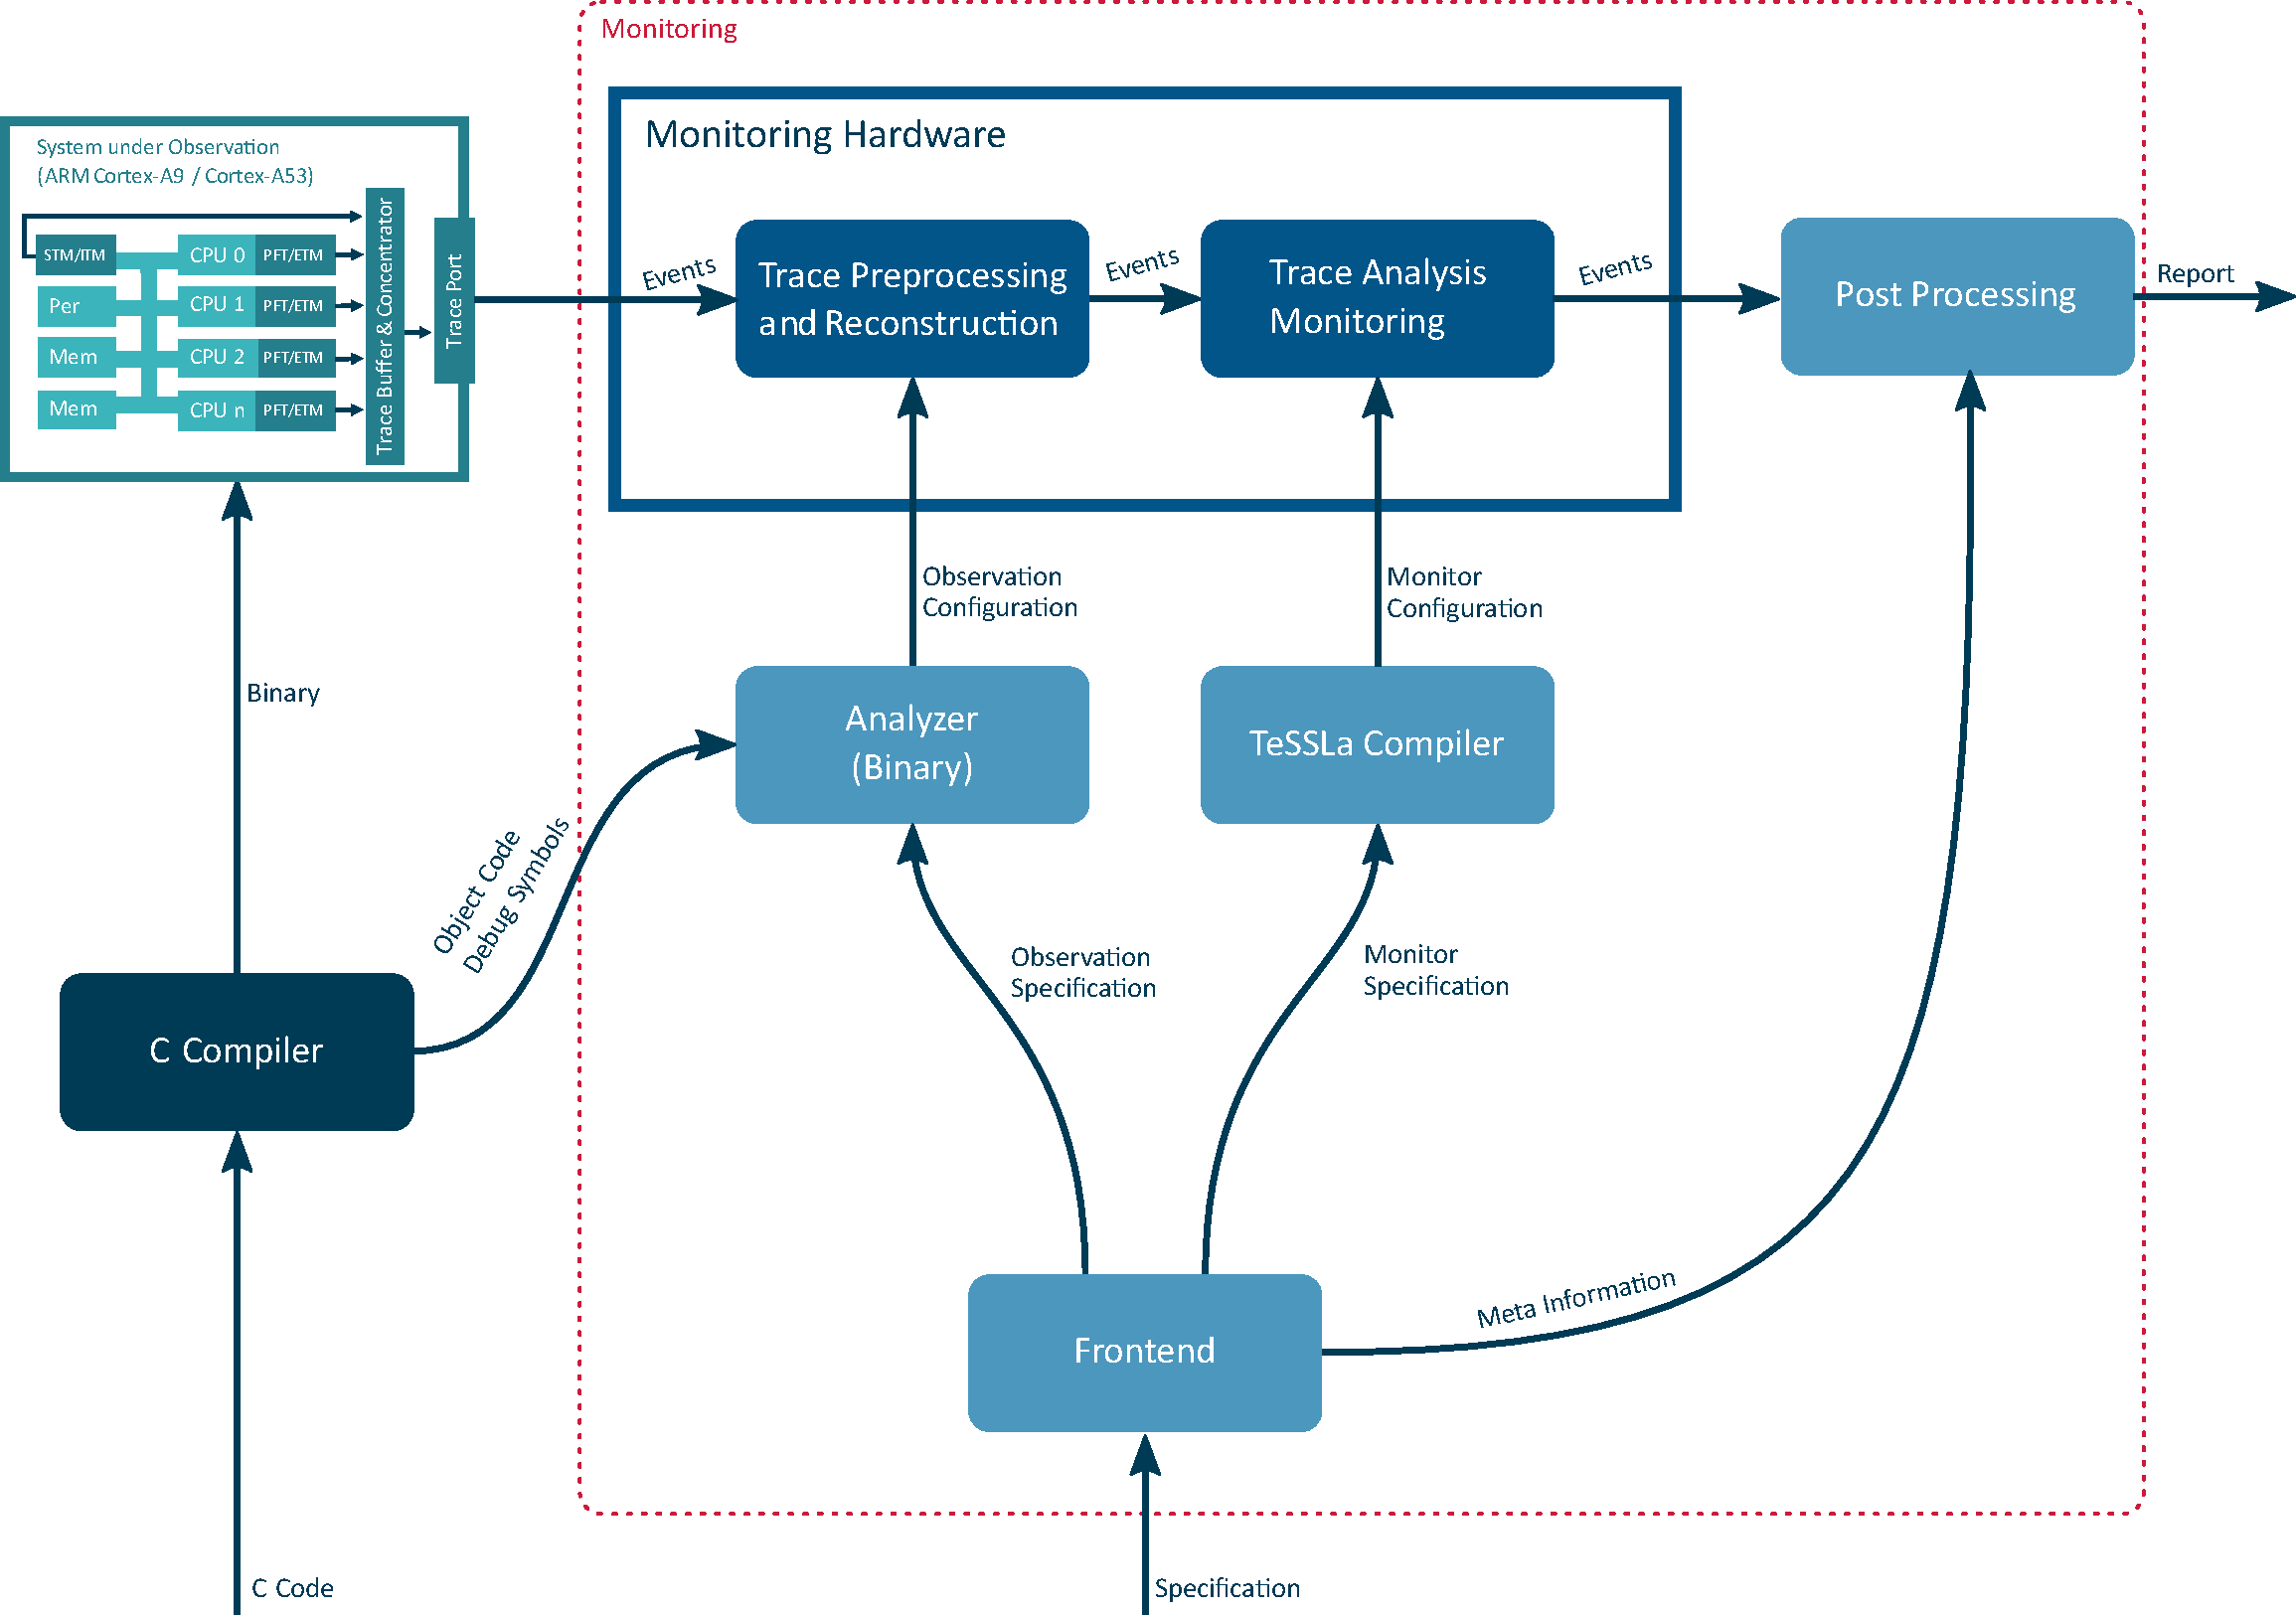
\includegraphics[width=.9\textwidth]{content/chapter_hardware_srv/overview-program-trace.pdf}
\end{frame}

\begin{frame}[plain]{Monitoring Data Values}
  \textwidthplain
  \centering
  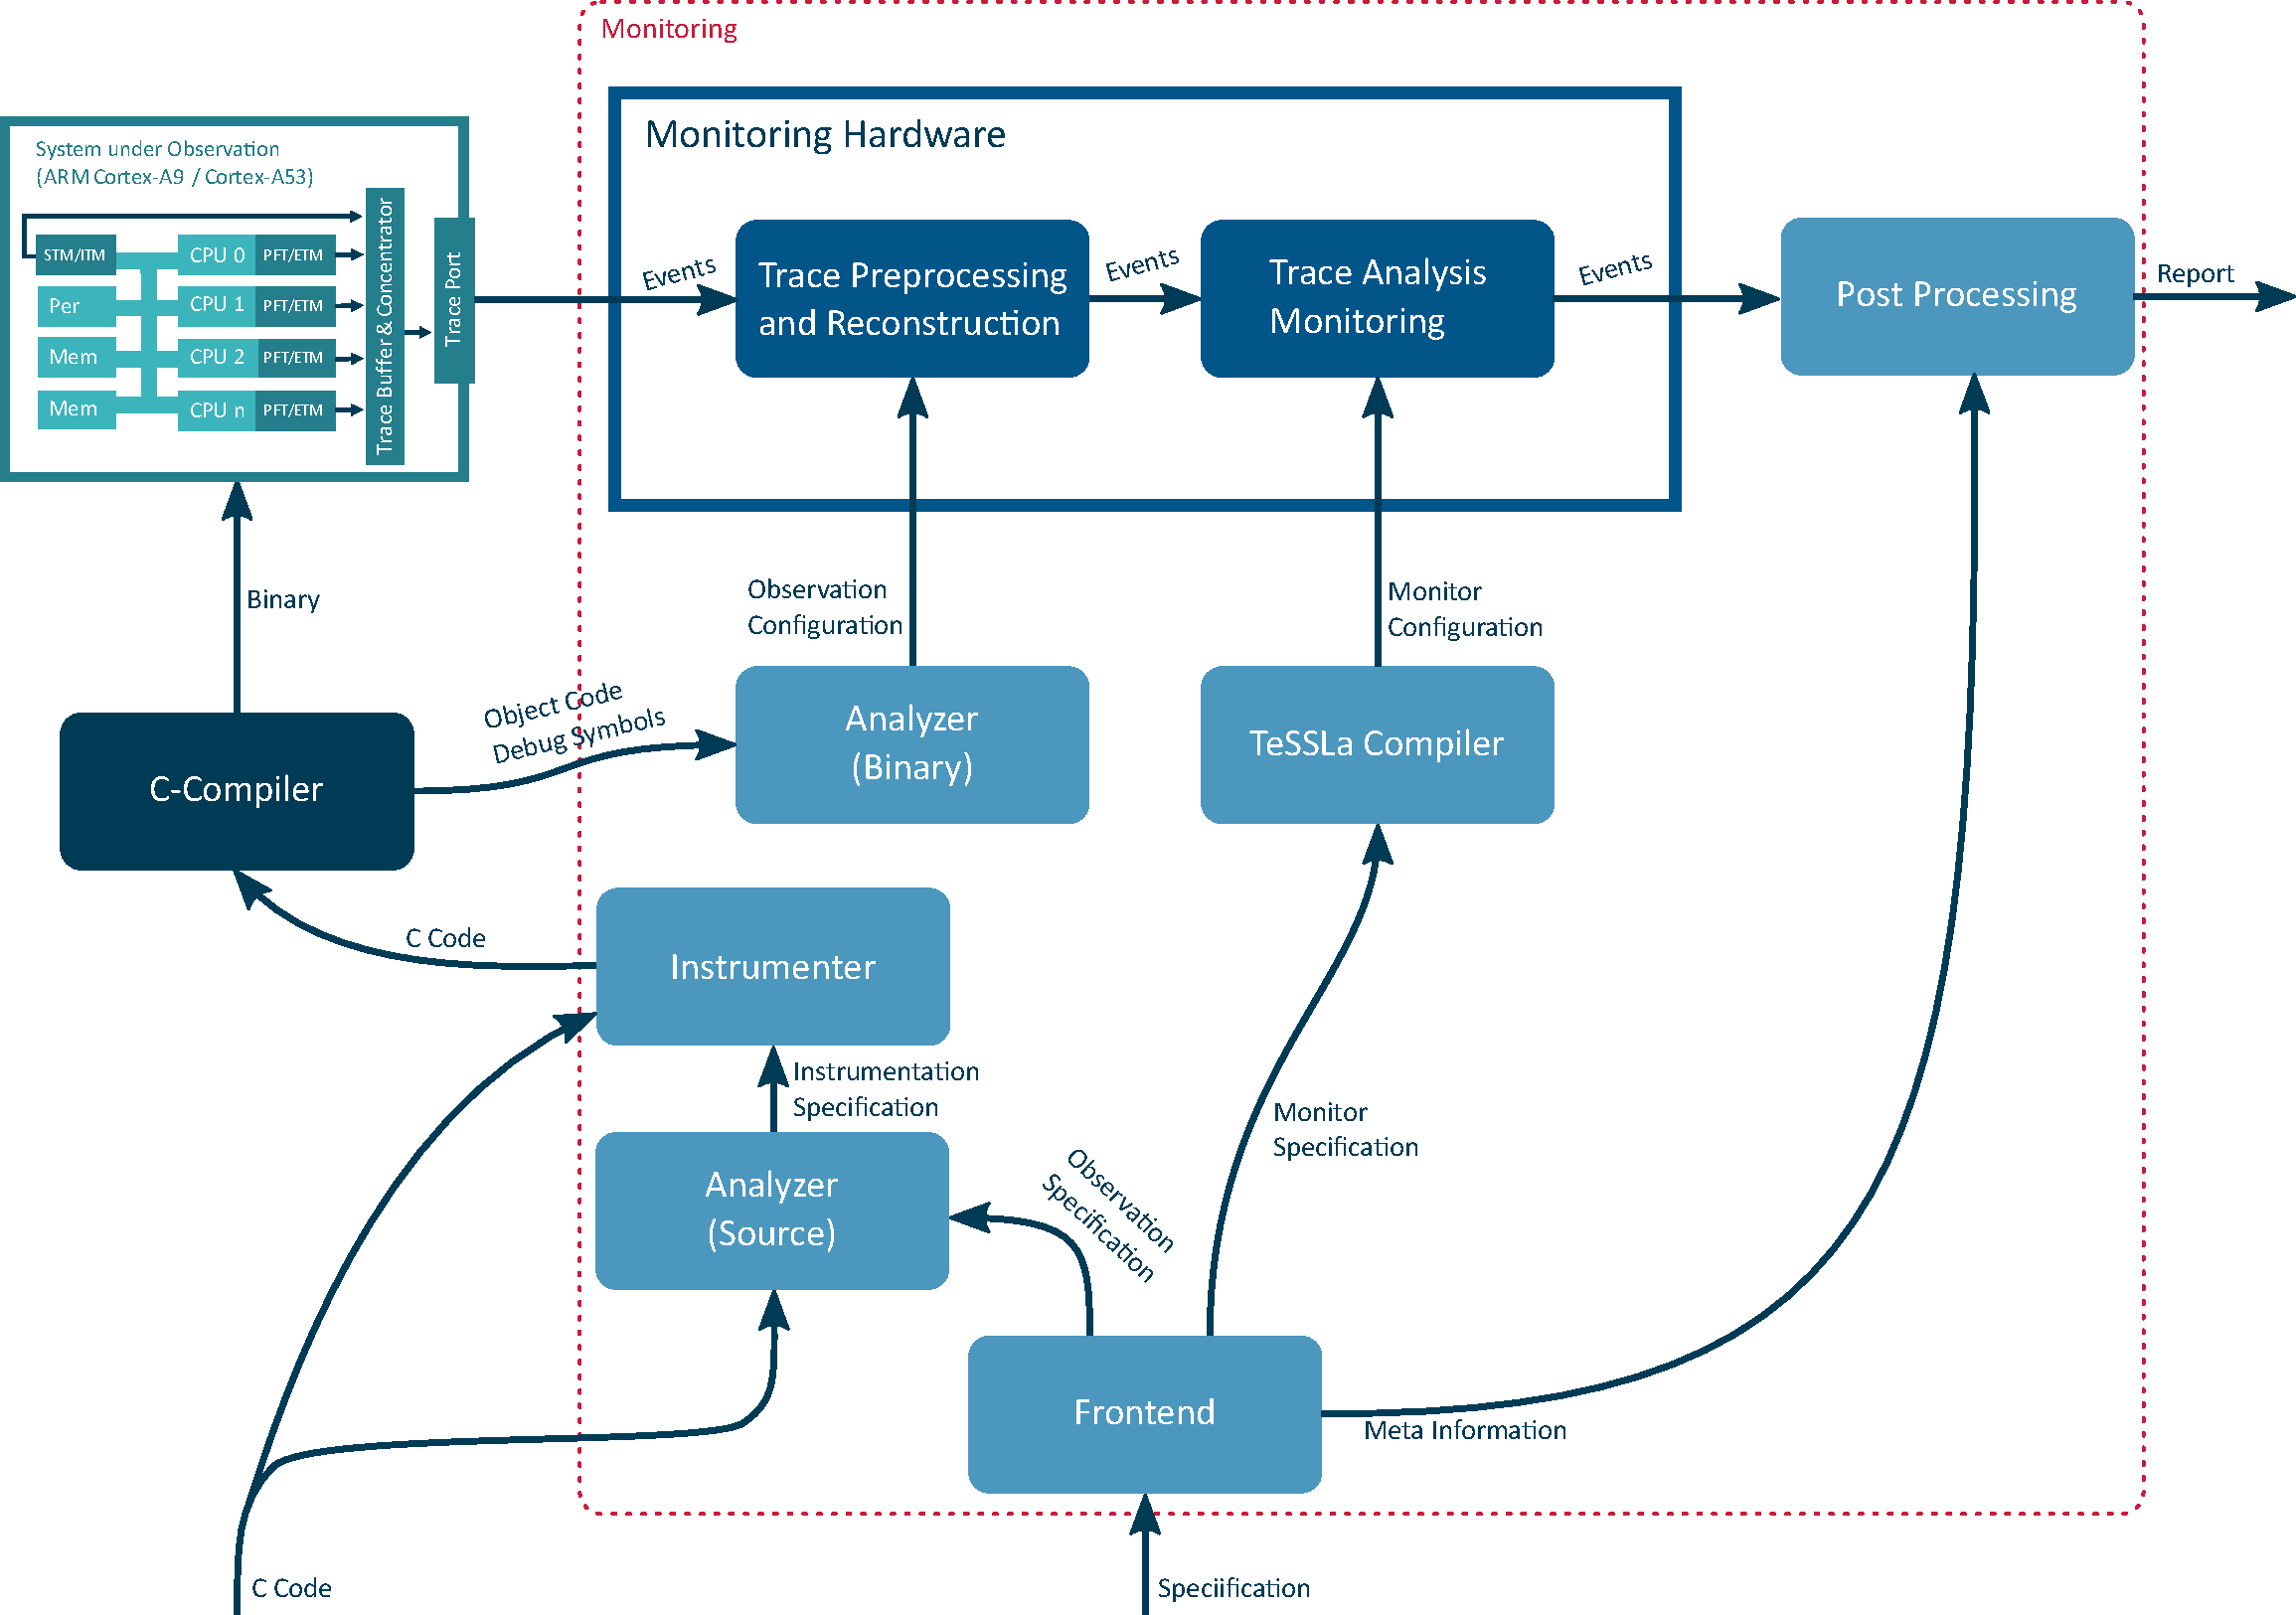
\includegraphics[width=.9\textwidth]{content/chapter_hardware_srv/overview-itm.pdf}
\end{frame}

\begin{frame}[fragile]{Monitoring the Speed Supervisor}
  \begin{block}{Property}
    23~s after the distant signal the allowed speed\\
    computed by the supervisor must be equal to 85~km/h.
  \end{block}

  \scriptsize

  \begin{lstlisting}[gobble=4,language=tessla]
    # Specify values we are interested in
    def signal := function_argument("getAllowedSpeed", 1)
    def allowed_speed := function_result("getAllowedSpeed")

    # Changes where signal becomes DISTANT_SIGNAL_CAUTION
    def caution := filter(changes(signal),
                        signal == DISTANT_SIGNAL_CAUTION)

    def valid :=
      # Either we are not yet 23s after the distant signal
      time(allowed_speed) - time(caution) <= 23s
      # or the allowed speed must be below 85~km/h
      || allowed_speed * 36 <= 85 * 1000
  \end{lstlisting}
\end{frame}

\begin{frame}[fragile]{Monitoring Data Value: How It Works}
  \scriptsize

  \begin{lstlisting}[gobble=4,language=tessla]
    # Specify values we are interested in
    def signal := function_argument("getAllowedSpeed", 1)
    def allowed_speed := function_result("getAllowedSpeed")
  \end{lstlisting}

  \xxx

  \begin{columns}
    \column{4.7cm}
    \inhead{Instrumented C Code}
    \vskip-3pt
      \begin{lstlisting}[gobble=6,language=C]
      double getAllowedSpeed(
          int signal, ...) {
        tessla_debug(1, (int64_t)
          signal);
        double result = ...
        tessla_debug(2, (int64_t)
          (result * 1000));
        return result;
      }
    \end{lstlisting}

    \column{4.7cm}
    \inhead{Updated Specification}
    \vskip-3pt
    \begin{lstlisting}[gobble=6,mathescape=true,language=tessla]
      in debug_slot: Events[Int]
      in debug_value: Events[Int]
      def signal :=
        filter(debug_value,
          debug_slot == 1)
      def allowed_speed :=
        filter(debug_value,
          debug_slot == 2)
          $~$
    \end{lstlisting}
  \end{columns}
\end{frame}


\section*{Conclusion}

\begin{frame}{Conclusion}
  \begin{enumerate}
    \item \alert{COEMS} provides \alert{interactive} debugging and \alert{continuous monitoring} for \alert{embedded and cyber-physical systems}.
    \item \alert{Continuous monitoring} of processor traces provided by \alert{embedded tracing units (ETU)} requires
      \begin{itemize}
        \item \alert{online trace reconstruction} in hardware and
        \item \alert{monitoring in hardware}.
      \end{itemize}
    \item Using \alert{TeSSLa} we can check
      \begin{itemize}
        \item \alert{event ordering} constraints,
        \item \alert{timing} constraints and
        \item \alert{complex event patterns} like the burst pattern.
      \end{itemize}
    \item TeSSLa can be used to \alert{aggregate data} and\\ compute \alert{statistical data}.
    \item Monitoring \alert{data values} is possible with \alert{lightweight instrumentation}.
      Specifications with data can be naturally written in TeSSLa.
  \end{enumerate}
\end{frame}